% Options for packages loaded elsewhere
\PassOptionsToPackage{unicode}{hyperref}
\PassOptionsToPackage{hyphens}{url}
%
\documentclass[
  a4paper,
]{article}
\usepackage{amsmath,amssymb}
\usepackage{setspace}
\usepackage{iftex}
\ifPDFTeX
  \usepackage[T1]{fontenc}
  \usepackage[utf8]{inputenc}
  \usepackage{textcomp} % provide euro and other symbols
\else % if luatex or xetex
  \usepackage{unicode-math} % this also loads fontspec
  \defaultfontfeatures{Scale=MatchLowercase}
  \defaultfontfeatures[\rmfamily]{Ligatures=TeX,Scale=1}
\fi
\usepackage{lmodern}
\ifPDFTeX\else
  % xetex/luatex font selection
\fi
% Use upquote if available, for straight quotes in verbatim environments
\IfFileExists{upquote.sty}{\usepackage{upquote}}{}
\IfFileExists{microtype.sty}{% use microtype if available
  \usepackage[]{microtype}
  \UseMicrotypeSet[protrusion]{basicmath} % disable protrusion for tt fonts
}{}
\makeatletter
\@ifundefined{KOMAClassName}{% if non-KOMA class
  \IfFileExists{parskip.sty}{%
    \usepackage{parskip}
  }{% else
    \setlength{\parindent}{0pt}
    \setlength{\parskip}{6pt plus 2pt minus 1pt}}
}{% if KOMA class
  \KOMAoptions{parskip=half}}
\makeatother
\usepackage{xcolor}
\usepackage[margin=1in]{geometry}
\usepackage{color}
\usepackage{fancyvrb}
\newcommand{\VerbBar}{|}
\newcommand{\VERB}{\Verb[commandchars=\\\{\}]}
\DefineVerbatimEnvironment{Highlighting}{Verbatim}{commandchars=\\\{\}}
% Add ',fontsize=\small' for more characters per line
\usepackage{framed}
\definecolor{shadecolor}{RGB}{248,248,248}
\newenvironment{Shaded}{\begin{snugshade}}{\end{snugshade}}
\newcommand{\AlertTok}[1]{\textcolor[rgb]{0.94,0.16,0.16}{#1}}
\newcommand{\AnnotationTok}[1]{\textcolor[rgb]{0.56,0.35,0.01}{\textbf{\textit{#1}}}}
\newcommand{\AttributeTok}[1]{\textcolor[rgb]{0.13,0.29,0.53}{#1}}
\newcommand{\BaseNTok}[1]{\textcolor[rgb]{0.00,0.00,0.81}{#1}}
\newcommand{\BuiltInTok}[1]{#1}
\newcommand{\CharTok}[1]{\textcolor[rgb]{0.31,0.60,0.02}{#1}}
\newcommand{\CommentTok}[1]{\textcolor[rgb]{0.56,0.35,0.01}{\textit{#1}}}
\newcommand{\CommentVarTok}[1]{\textcolor[rgb]{0.56,0.35,0.01}{\textbf{\textit{#1}}}}
\newcommand{\ConstantTok}[1]{\textcolor[rgb]{0.56,0.35,0.01}{#1}}
\newcommand{\ControlFlowTok}[1]{\textcolor[rgb]{0.13,0.29,0.53}{\textbf{#1}}}
\newcommand{\DataTypeTok}[1]{\textcolor[rgb]{0.13,0.29,0.53}{#1}}
\newcommand{\DecValTok}[1]{\textcolor[rgb]{0.00,0.00,0.81}{#1}}
\newcommand{\DocumentationTok}[1]{\textcolor[rgb]{0.56,0.35,0.01}{\textbf{\textit{#1}}}}
\newcommand{\ErrorTok}[1]{\textcolor[rgb]{0.64,0.00,0.00}{\textbf{#1}}}
\newcommand{\ExtensionTok}[1]{#1}
\newcommand{\FloatTok}[1]{\textcolor[rgb]{0.00,0.00,0.81}{#1}}
\newcommand{\FunctionTok}[1]{\textcolor[rgb]{0.13,0.29,0.53}{\textbf{#1}}}
\newcommand{\ImportTok}[1]{#1}
\newcommand{\InformationTok}[1]{\textcolor[rgb]{0.56,0.35,0.01}{\textbf{\textit{#1}}}}
\newcommand{\KeywordTok}[1]{\textcolor[rgb]{0.13,0.29,0.53}{\textbf{#1}}}
\newcommand{\NormalTok}[1]{#1}
\newcommand{\OperatorTok}[1]{\textcolor[rgb]{0.81,0.36,0.00}{\textbf{#1}}}
\newcommand{\OtherTok}[1]{\textcolor[rgb]{0.56,0.35,0.01}{#1}}
\newcommand{\PreprocessorTok}[1]{\textcolor[rgb]{0.56,0.35,0.01}{\textit{#1}}}
\newcommand{\RegionMarkerTok}[1]{#1}
\newcommand{\SpecialCharTok}[1]{\textcolor[rgb]{0.81,0.36,0.00}{\textbf{#1}}}
\newcommand{\SpecialStringTok}[1]{\textcolor[rgb]{0.31,0.60,0.02}{#1}}
\newcommand{\StringTok}[1]{\textcolor[rgb]{0.31,0.60,0.02}{#1}}
\newcommand{\VariableTok}[1]{\textcolor[rgb]{0.00,0.00,0.00}{#1}}
\newcommand{\VerbatimStringTok}[1]{\textcolor[rgb]{0.31,0.60,0.02}{#1}}
\newcommand{\WarningTok}[1]{\textcolor[rgb]{0.56,0.35,0.01}{\textbf{\textit{#1}}}}
\usepackage{graphicx}
\makeatletter
\def\maxwidth{\ifdim\Gin@nat@width>\linewidth\linewidth\else\Gin@nat@width\fi}
\def\maxheight{\ifdim\Gin@nat@height>\textheight\textheight\else\Gin@nat@height\fi}
\makeatother
% Scale images if necessary, so that they will not overflow the page
% margins by default, and it is still possible to overwrite the defaults
% using explicit options in \includegraphics[width, height, ...]{}
\setkeys{Gin}{width=\maxwidth,height=\maxheight,keepaspectratio}
% Set default figure placement to htbp
\makeatletter
\def\fps@figure{htbp}
\makeatother
\setlength{\emergencystretch}{3em} % prevent overfull lines
\providecommand{\tightlist}{%
  \setlength{\itemsep}{0pt}\setlength{\parskip}{0pt}}
\setcounter{secnumdepth}{-\maxdimen} % remove section numbering
\ifLuaTeX
\usepackage[bidi=basic]{babel}
\else
\usepackage[bidi=default]{babel}
\fi
\babelprovide[main,import]{catalan}
% get rid of language-specific shorthands (see #6817):
\let\LanguageShortHands\languageshorthands
\def\languageshorthands#1{}
\ifLuaTeX
  \usepackage{selnolig}  % disable illegal ligatures
\fi
\usepackage{bookmark}
\IfFileExists{xurl.sty}{\usepackage{xurl}}{} % add URL line breaks if available
\urlstyle{same}
\hypersetup{
  pdfauthor={@tofermos 2024},
  pdflang={ca-ES},
  hidelinks,
  pdfcreator={LaTeX via pandoc}}

\title{Software. Instal·lar i desinstal·lar.}
\author{@tofermos 2024}
\date{}

\begin{document}
\maketitle

{
\setcounter{tocdepth}{2}
\tableofcontents
}
\setstretch{1.5}
\newpage

\renewcommand\tablename{Tabla}

\section{1 INSTAL·LACIÓ}\label{installaciuxf3}

\subsection{1.1 FITXERS MSI}\label{fitxers-msi}

Els fitxers amb extensió MSI ( Microsoft Installer) son paquets per a
instal·lació , desinstal·lació i manteniment de softwarer ne sistemes
Windows.

Des del GUI podem executar com adminsitrador i instal·lar. Des del CLI,
cmd, veiem com sería la instal·lació:

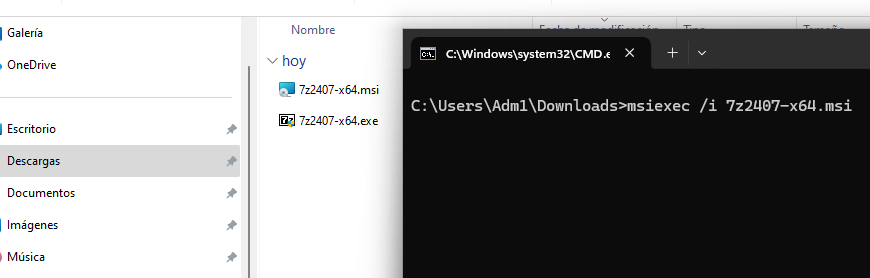
\includegraphics{png/instalarMSIcmd.png}

\begin{Shaded}
\begin{Highlighting}[]
\NormalTok{msiexec }\AttributeTok{/i}\NormalTok{ 7z2407}\AttributeTok{{-}x64}\NormalTok{.msi}
\end{Highlighting}
\end{Shaded}

Comença la instal·lació

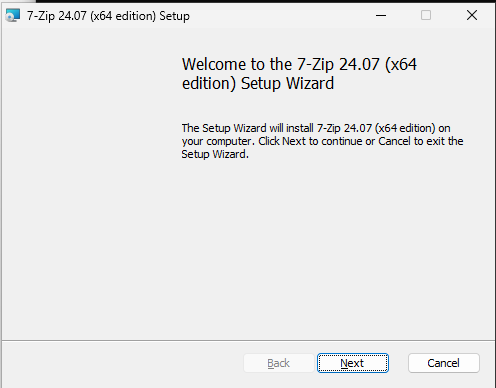
\includegraphics{png/instalarMSIcmd1.png}

Ens informa i demana consentiment de la llicència.
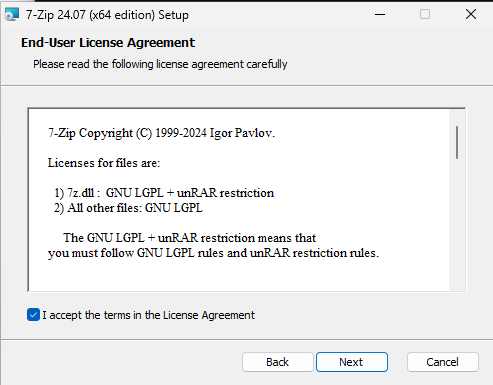
\includegraphics{png/instalarMSI2.png}

Per defecte s'instal·la en ``C:\textbackslash Program Files'' però
normalment podríem canviar la carpeta destí de la instal·lació.

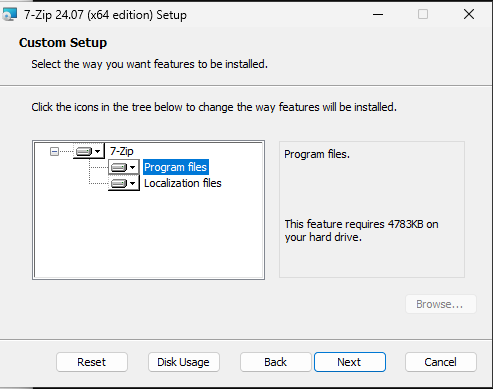
\includegraphics{png/instalarMSI3.png}

El SO ens avisa de l'intent de instal·lar-se i ens demana autorització.
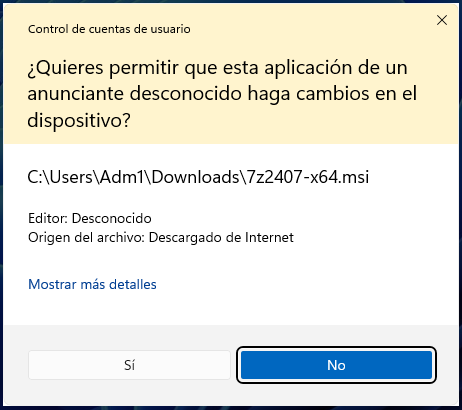
\includegraphics{png/instalarMSI4.png}

Una vegada finalitzada la instal·lació, comprovem que existeix i provem
el programa. Molt sovint, al final de la instal·lació se'ns demana
reiniciar el PC.

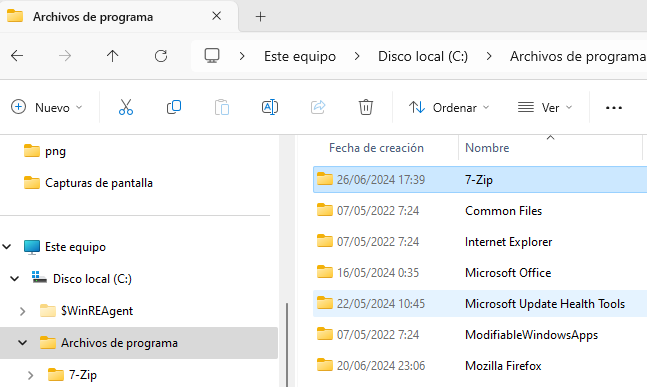
\includegraphics{png/instalarMSI5.png}

\subsection{1.2 FITXERS .EXE}\label{fitxers-.exe}

Els fitxers amb extensió \emph{.exe} són executables de programes amb
moltes possibles funcions. Des d'aplicacions d'usuari (calc.exe,
winword.exe), components del sistema operatiu (regedit.exe,
netplwiz.exe); eines com IDE per a programar (android-studio-2023.1.ex,
VSCodeSetup-x64-1.72.0.exe ); eines per a l'execució de codi com
intérprets, màquines virtuals\ldots{}

El que ens interessa ara són el .exe que serveixen per instalar
software. A diferència del .msi, no necessiten cap altre programa i
només cal executar-los com a administrador. Solne tindre noms com
``installer.exe'' o ``setup.exe''.

\subsection{1.3 FITXERS .inf PER INSTAL·LAR I CONFIGURAR DISPOSITIUS
HARDWARE}\label{fitxers-.inf-per-installar-i-configurar-dispositius-hardware}

No són fitxers amb codi executable. Sinó que contenen informació de text
pla (caràters llegibles i editable per nosaltres) amb informació sobre
el controlador d'un dipositiu que Windows llig per a instal·lar-lo.

Exemple:

\begin{verbatim}
[Version]
Signature="$Windows NT$"
Class=Printer
ClassGuid={4D36E979-E325-11CE-BFC1-08002BE10318}
Provider=%ProviderName%
DriverVer=07/01/2021,1.0.0.0

[Manufacturer]
%ManufacturerName%=PrinterManufacturer,NTamd64

[PrinterManufacturer.NTamd64]
%ModelName%=Install,USBPRINT\PrinterModel

[Install]
CopyFiles=@PrinterDriver.dll
AddReg=PrinterAddReg

[PrinterAddReg]
HKR,,PortNumber,,"USB001"

[SourceDisksNames]
1 = %DiskName%,,,""
...
\end{verbatim}

\subsection{1.4 ALTRES}\label{altres}

\subsubsection{bat (Batch File) i .cmd}\label{bat-batch-file-i-.cmd}

Arxiu script que puede ejecutar comandaments de Windwos. S'usa poc hui
en dia i només en instal·lacions senzilles. Nom típic:
\emph{install.bat}

Els .cmd son similars a .bat, pero executats pel cmd.exe. Exemple:
\emph{install.cmd}

\subsubsection{.msix/.appx}\label{msix.appx}

Formatos més recents Microsoft per empaquetar aplicacions de la Botiga
de Windows. Exemples: appinstaller.msix, application.appx.

\section{2 DESINSTAL·LACIÓ}\label{desinstallaciuxf3}

Qualsevol desinstal·lació d'un programa ens obligarà a tancar-lo com a
primer pas. Una vegada tancat veiem diverses formes de desinstal·lar,
modificar o reparar la instal·lacio d'un programa.

\subsection{2.1 DESDE l'APPLET DEL PANEL DE
CONTROL}\label{desde-lapplet-del-panel-de-control}

Com ja anem veient, al GUI de Windows, hi ha molts ``camins diferents''
per arribar al mateix lloc quan l'objectiu final és l'execució d'un
component de Windows o un programa instal·lat. En el nostre cas burcarem
el component o ferramenta per a desinstal·lar programes.

\textbf{Per entrar al \emph{Panel de control} } Des del menú de Windows
( Win +S o Win i escrivint ``panel\ldots{}'') o executant Win+R: control

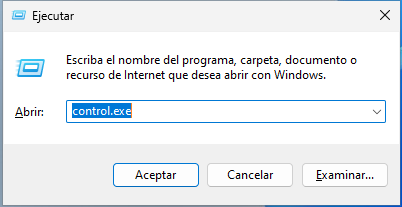
\includegraphics{png/control-exe.png}

\textbf{i ja per desinstal·lar o modificar la instal·lació d'un
programa\ldots{}} Seleccionem \textbf{Programas y características}. Este
element de Windows, a banda de modificar i eliminar una instal·lació,
ens permet veure caraterístiques com l'espai del disc dur que ocupa la
instal·lació.

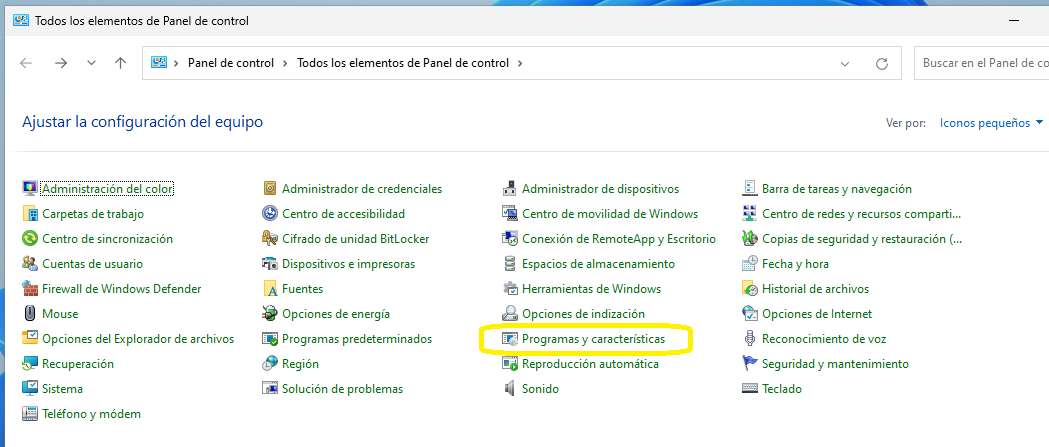
\includegraphics{png/paneldeControl.png}

Seleccionen el programa a desinstal·lar o canviar i amb el botó contrari
triem l'opció que volem:

\begin{itemize}
\tightlist
\item
  Desinstal·lar el programa. Pot demanar-nos (i és recomanable)
  reiniciar l'equip en acabar.
\item
  Fer algun canvi en la instal·lació existent.
\item
  Reparar a instal·lació. Pot demanar-nos els fitxers originals de la
  instal·lació.
\end{itemize}

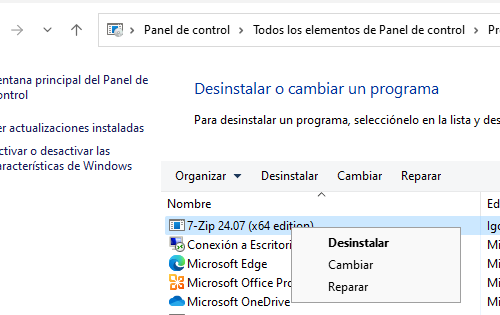
\includegraphics{png/programasycaracteristicasDesinstalar.png}

Ens tornarà a advertir de l'intent de modificar el software i demanarà
autorització.

\textbf{Avanç}

\begin{quote}
Els Applets del Panel de Control són components, com este que estem
veient, que tenen extensió \emph{.cpl}. Poden executar-se directament:
\end{quote}

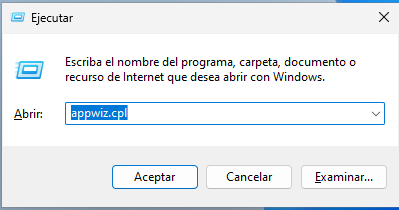
\includegraphics{png/appwiz-cpl.png}

\subsection{2.2 AMB .MSI}\label{amb-.msi}

Si la instal·lació sha fet a partir d'un fitxer \emph{.msi}, tal com hem
comentat, els fitxer MSI serveixen no sols per instal·lar, també per
desintal·lar.

\begin{Shaded}
\begin{Highlighting}[]
\NormalTok{msiexec }\AttributeTok{/x}\NormalTok{ 7z2407}\AttributeTok{{-}x64}\NormalTok{.msi}
\end{Highlighting}
\end{Shaded}

Però el més habitual és que ja no conservem el .msi. En este cas,
necessitarem esbrinar l'identificador de programa buscant pel nom del
programa dins del Registre de Windows (Win+R regedit.exe)
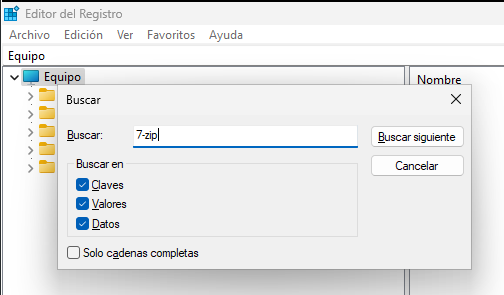
\includegraphics{png/buscaralRegistre.png}

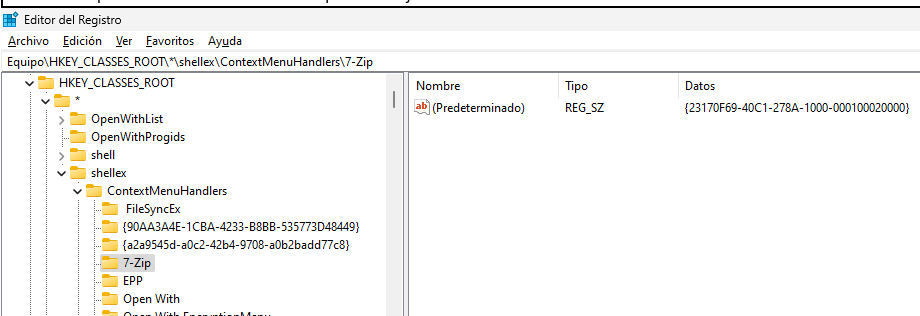
\includegraphics{png/productCodeRegedit.png}

Alternativament podríem fer ús de l'eina WIMC. De moment no ho
estudiarem.

\begin{Shaded}
\begin{Highlighting}[]
\NormalTok{wmic product get Name, identifyingnumber}
\end{Highlighting}
\end{Shaded}

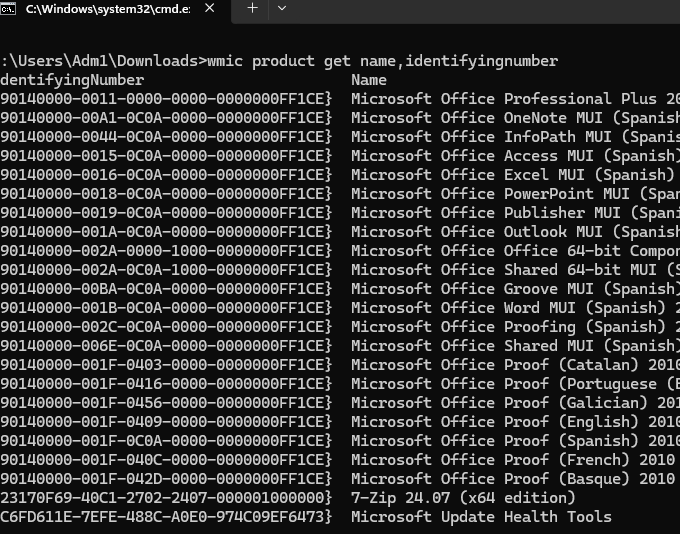
\includegraphics{png/desinstalarMSI1.png}

O de PowerShell. De moment no ho estudiarem.

\begin{Shaded}
\begin{Highlighting}[]
\FunctionTok{Get{-}WmiObject} \OperatorTok{{-}}\NormalTok{Class Win32\_Product }\OperatorTok{|} \FunctionTok{Select{-}Object}\NormalTok{ Name}\OperatorTok{,}\NormalTok{ IdentifyingNumber}
\end{Highlighting}
\end{Shaded}

Una vegada sabem el GUID de la instal·lació ja podem fer la
desinstal·lació.

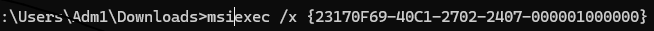
\includegraphics{png/desinstalarMSI2.png}

\begin{Shaded}
\begin{Highlighting}[]
\NormalTok{msiexec }\AttributeTok{/x}\NormalTok{ \{ GUID \}}
\end{Highlighting}
\end{Shaded}

\section{3 INTEGRITAT DELS PAQUETS}\label{integritat-dels-paquets}

Molt sovint els fabricants de software posen a la nostra disposició la
possibilitat de comprovar si la descàrrega d'un fitxer s'ha fet
correctament (verificar la integritat del fitxer, que no hi haja cap
bloc corrupte). Sobretot quan el tamany del fitxer és elevat. És el cas
dels fitxer ISO de molts paquets de software i, concretament, dels
Sistemes Operatius.

Per a tal cosa, se'ns aporta un codi que és el resultat d'aplicar una
funció al conjunt de bits que formen el fitxer. Nosaltres el que hem de
fer és aplicar la mateixa funció al fitxer descarregat i comprovar que
ens dona el mateix número.

\subsection{3.1 Funció SHA256}\label{funciuxf3-sha256}

SHA-256 o Secure Hash Algorithm 256 bits és una función hash
criptográfica que genera un valor hash único per a un fitxer. S'usa per
a verificar la integritat de les dades assegurant que no hi ha haguts
canvis entre el fitxer final i l'original en una còpia, descàrrega,
enviament\ldots{}

El powershell no cal dominar-lo encara però és interessant que conegam
que implementa funcions com esta.

\begin{Shaded}
\begin{Highlighting}[]
\NormalTok{Get{-}FileHash C}\OperatorTok{:}\NormalTok{\textbackslash{}Users\textbackslash{}Adm1\textbackslash{}Downloads\textbackslash{}FitxerDescarregat}\OperatorTok{.}\FunctionTok{iso}
\end{Highlighting}
\end{Shaded}

\subsection{3.2 Comprovació de la ISO del Windows
11.}\label{comprovaciuxf3-de-la-iso-del-windows-11.}

\begin{enumerate}
\def\labelenumi{\arabic{enumi}.}
\tightlist
\item
  Seleccionem la ISO que necessitem: 64 bits, Español- España.
\end{enumerate}

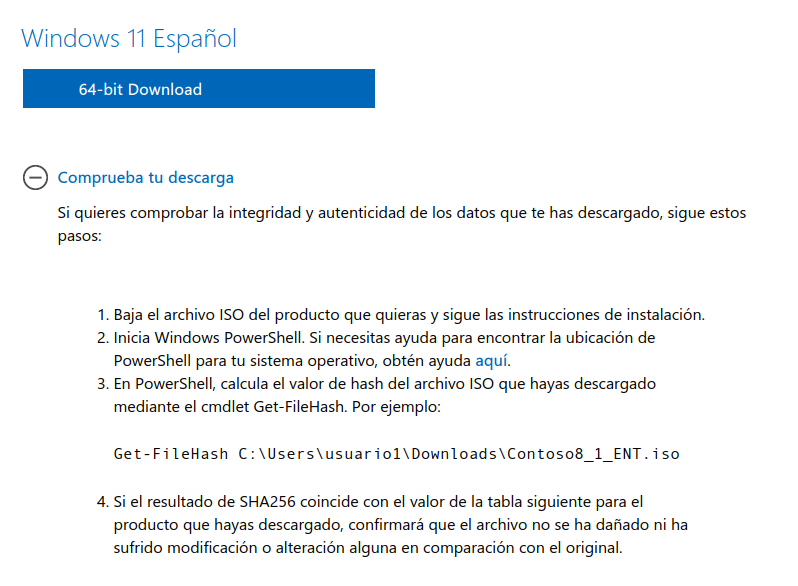
\includegraphics{png/comprobarSHA1.png}

\begin{enumerate}
\def\labelenumi{\arabic{enumi}.}
\setcounter{enumi}{1}
\tightlist
\item
  Anotem el codi SHA256 que ens ha de donar. en este cas la funció que
  Microsoft ha usat el la SHA256
\end{enumerate}

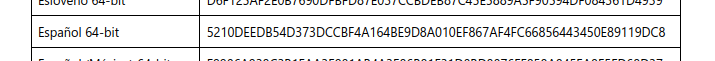
\includegraphics{png/comprobarSHA2.png}

\begin{enumerate}
\def\labelenumi{\arabic{enumi}.}
\setcounter{enumi}{2}
\tightlist
\item
  Obrim el Powershell i ens situem en la carpeta on està la ISO i
  executem la funció.
\end{enumerate}

(si tenim dificultats per moure'ns amb els cmdLets, podem situar-nos en
la carpeta abans d'executar la funció GetHash)

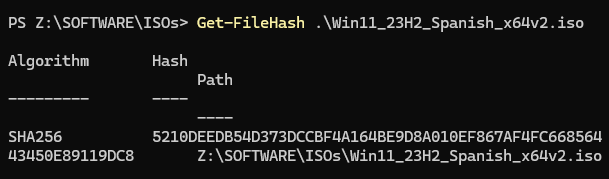
\includegraphics{png/getHash1.png}

\begin{enumerate}
\def\labelenumi{\arabic{enumi}.}
\setcounter{enumi}{3}
\tightlist
\item
  Comprovem a colp de vista (almenys) que els codis coincideixen. En cas
  contrari hem tingut algun problema desant el fitxer: la ISO no sería
  vàlida.
\end{enumerate}

\section{4 ACTIVITATS}\label{activitats}

\section{4.1 Instal·lació des de .exe}\label{installaciuxf3-des-de-.exe}

\begin{enumerate}
\def\labelenumi{\arabic{enumi}.}
\item
  Descarrega el Opera.exe per a Windows 64 bits
  \url{https://www.opera.com/es/download}
\item
  Instal·la'l.
\item
  Averigua en quins directoris està instal·lat.
\end{enumerate}

\subsection{4.2 Instal·lació des d'un
.msi}\label{installaciuxf3-des-dun-.msi}

\begin{enumerate}
\def\labelenumi{\arabic{enumi}.}
\tightlist
\item
  Descarrega't el paquet d'instal·lació del navegador Firefox en msi en
  valencià de la web:
\end{enumerate}

\url{https://www.mozilla.org/es-ES/firefox/all/\#product-desktop-release}

Fixeu-vos en triar l'opció de 64bits i MSI

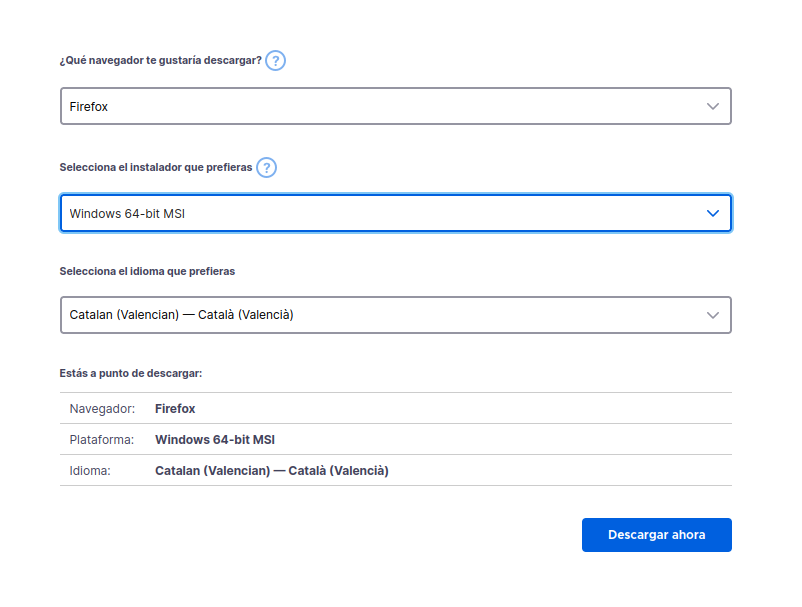
\includegraphics{png/firefoxDescarregaMSI.png}

\begin{enumerate}
\def\labelenumi{\arabic{enumi}.}
\setcounter{enumi}{1}
\item
  Instal·la des del cmd.
\item
  Mira en quins directoris de Windows s'ha instal·lat.
\item
  Investiga quin dels dos navegadors (FireFox i Opera) ocupa més espai
  al disc dur.
\item
  Busca al registre de Windows el GUID
\item
  Elimina el fitxer .msi
\item
  Desinstal·la el FireFox des de cmd usant l'identificador identificador
  GUID.
\end{enumerate}

\subsection{4.3 Comprovació SHA256}\label{comprovaciuxf3-sha256}

\begin{enumerate}
\def\labelenumi{\arabic{enumi}.}
\tightlist
\item
  Descarrega't un Windows 11 per al teu PC particular o portàtil.
\item
  Comprova que la ISO descarregada és vàlida.
\end{enumerate}

\end{document}
